\documentclass[11pt]{amsart}

\usepackage[T1]{fontenc}
\usepackage{lmodern}
\usepackage{microtype}
\usepackage{amsmath,amssymb}
\usepackage{booktabs}
\usepackage{tikz}
\usetikzlibrary{arrows.meta}
\usepackage[hidelinks]{hyperref}

\hypersetup{
  pdftitle={A Five-Vertex Counterexample to Conjecture 5.8 of Curto, Geneson, and Morrison}
}

\newtheorem{theorem}{Theorem}
\newtheorem{lemma}[theorem]{Lemma}

\newcommand{\one}{\mathbf{1}}
\newcommand{\eps}{\varepsilon}

\title[A five-vertex counterexample]
{A Five-Vertex Counterexample to Conjecture 5.8 of Curto, Geneson, and Morrison}

\date{}

\keywords{combinatorial threshold-linear network, permitted motif,
composite graph, counterexample}

\begin{document}

\begin{abstract}
We refute the reverse implication of Conjecture~5.8 of Curto,
Geneson, and Morrison concerning permitted motifs in composite CTLNs.
We exhibit a five-vertex composite graph whose skeleton and all four
components are permitted, whereas the full graph is forbidden, for every
legal parameter choice. The construction is uniformly nondegenerate, and
five vertices is the minimum possible order of such a counterexample.
\end{abstract}

\maketitle

\section{The counterexample}

For a directed graph $G$, the associated combinatorial threshold-linear
network has connectivity matrix
\[
W_{ij}=
\begin{cases}
0, & i=j,\\
-1+\eps, & j\to i,\\
-1-\delta, & j\not\to i,
\end{cases}
\qquad
\theta>0,\quad \delta>0,\quad
0<\eps<\frac{\delta}{\delta+1}.
\]
We follow the standing nondegeneracy convention of \cite{CGM}. Thus the
full vertex set is a permitted motif precisely when the solution of
\[
(I-W_G)x=\theta\one
\]
is strictly positive.

A composite graph is obtained by replacing each vertex of a skeleton by
a component graph and inserting all intercomponent edges prescribed by
the skeleton. Conjecture~5.8 of \cite{CGM} states that if the skeleton is
permitted, then the composite graph is permitted if and only if every
component is permitted. The forward implication is Theorem~5.2 of
\cite{CGM}. Recent work gives a one-way compositionality theorem for
low-rank gluings and a complete survival characterization for the
rank-$1$ subclass \cite{LA}; the construction below is not rank~$1$,
because vertices of $G_B$ project differently to $G_A$ and $G_C$.

\begin{theorem}\label{thm:counterexample}
There exists a composite graph $G$ on five vertices such that, for every
legal choice of $(\eps,\delta,\theta)$, its skeleton and all four
components are permitted motifs, whereas the full vertex set of $G$ is
forbidden. The CTLNs on $G$, its skeleton, and its components are
nondegenerate throughout the legal parameter region. Consequently, the
reverse implication in Conjecture~5.8 of \cite{CGM} is false.
\end{theorem}

\begin{proof}
Let the skeleton $\widehat G$ have vertices $A,B,C,D$ and edges
\[
A\leftrightarrow D,
\qquad
B\leftrightarrow C,
\qquad
B\to D,
\qquad
C\to A.
\]
Here $K_m$ denotes the bidirected clique on $m$ vertices. Take
\[
G_A=K_1,
\qquad
G_B=K_2,
\qquad
G_C=K_1,
\qquad
G_D=K_1.
\]
Writing the vertices of $G$ as $a,b_1,b_2,c,d$, its edges are
\[
a\leftrightarrow d,
\qquad
b_1\leftrightarrow b_2,
\qquad
b_i\leftrightarrow c,
\qquad
b_i\to d\quad(i=1,2),
\qquad
c\to a.
\]

\begin{figure}[t]
\centering
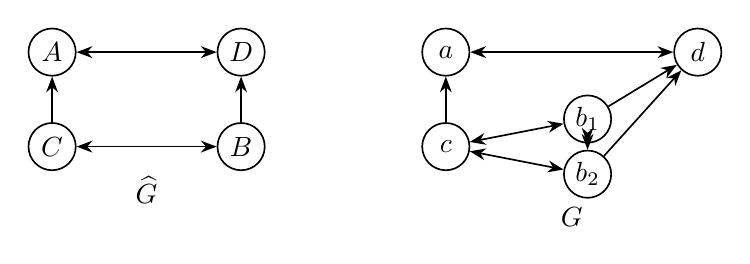
\begin{tikzpicture}[
  >=Stealth,
  vertex/.style={circle,draw,minimum size=6mm,inner sep=0pt},
  every path/.style={semithick}
]
\begin{scope}[xshift=-3.2cm]
  \node[vertex] (A) at (0,1.2) {$A$};
  \node[vertex] (D) at (2.4,1.2) {$D$};
  \node[vertex] (C) at (0,0) {$C$};
  \node[vertex] (B) at (2.4,0) {$B$};
  \draw[<->] (A)--(D);
  \draw[<->] (B)--(C);
  \draw[->] (B)--(D);
  \draw[->] (C)--(A);
  \node at (1.2,-0.55) {$\widehat G$};
\end{scope}
\begin{scope}[xshift=1.8cm]
  \node[vertex] (a) at (0,1.2) {$a$};
  \node[vertex] (d) at (3.2,1.2) {$d$};
  \node[vertex] (c) at (0,0) {$c$};
  \node[vertex] (b1) at (1.8,0.35) {$b_1$};
  \node[vertex] (b2) at (1.8,-0.35) {$b_2$};
  \draw[<->] (a)--(d);
  \draw[->] (c)--(a);
  \draw[<->] (c)--(b1);
  \draw[<->] (c)--(b2);
  \draw[<->] (b1)--(b2);
  \draw[->] (b1)--(d);
  \draw[->] (b2)--(d);
  \node at (1.6,-0.9) {$G$};
\end{scope}
\end{tikzpicture}
\caption{The permitted skeleton $\widehat G$ and its five-vertex
composite graph $G$. The component $G_B$ consists of $b_1,b_2$; the
other components are singletons.}
\label{fig:graphs}
\end{figure}

Set
\[
\alpha=1-\eps,
\qquad
\beta=1+\delta.
\]
In the orders $(A,B,C,D)$ and $(a,b_1,b_2,c,d)$, respectively,
\[
I-W_{\widehat G}=
\begin{pmatrix}
1&\beta&\alpha&\alpha\\
\beta&1&\alpha&\beta\\
\beta&\alpha&1&\beta\\
\alpha&\alpha&\beta&1
\end{pmatrix},
\]
and
\[
I-W_G=
\begin{pmatrix}
1&\beta&\beta&\alpha&\alpha\\
\beta&1&\alpha&\alpha&\beta\\
\beta&\alpha&1&\alpha&\beta\\
\beta&\alpha&\alpha&1&\beta\\
\alpha&\alpha&\alpha&\beta&1
\end{pmatrix}.
\]
Define
\begin{align*}
\widehat h
&=2\delta^2-2\delta\eps+6\delta-\eps^2+2\eps,\\
h
&=3\delta^2-3\delta\eps+9\delta-2\eps^2+4\eps.
\end{align*}
Direct multiplication verifies
\[
(I-W_{\widehat G})^{-1}\theta\one
=
\frac{\theta}{\widehat h}
\begin{pmatrix}
\delta\\
2\delta+\eps\\
2\delta+\eps\\
\delta
\end{pmatrix},
\qquad
\det(I-W_{\widehat G})=-\eps^2\widehat h,
\]
and
\[
(I-W_G)^{-1}\theta\one
=
\frac{\theta}{\eps h}
\begin{pmatrix}
-\delta^2\\
\eps(2\delta+\eps)\\
\eps(2\delta+\eps)\\
\eps(2\delta+\eps)\\
\delta^2+3\delta\eps+\eps^2
\end{pmatrix},
\qquad
\det(I-W_G)=-\eps^3h.
\]
The legal inequalities imply $0<\eps<\min\{\delta,1\}$, and hence
\[
\widehat h
=2\delta(\delta-\eps)+6\delta+\eps(2-\eps)>0,
\]
\[
h
=3\delta(\delta-\eps)+9\delta+2\eps(2-\eps)>0.
\]
Thus $\widehat G$ is permitted, whereas the first coordinate of the
full-support solution for $G$ is negative. Hence $G$ is forbidden.

The only nontrivial component is $K_2$, whose full-support solution is
\[
\frac{\theta}{2-\eps}(1,1)>0.
\]
Thus every component is permitted. Uniform nondegeneracy is proved in
Appendix~\ref{app:nondeg}.
\end{proof}

\section{Minimality}

The next reduction records the only information about a permitted
component needed by the skeleton.

\begin{lemma}\label{lem:reduction}
Let $G$ be a composite graph with nonempty permitted components
$G_1,\dots,G_N$, and suppose each $I-W_{G_i}$ is nonsingular. Put
\[
\alpha=1-\eps,
\qquad
\beta=1+\delta,
\]
and, for each $i$,
\[
y_i=(I-W_{G_i})^{-1}\one,
\qquad
T_i=\one^{\mathsf T}y_i,
\qquad
d_i=T_i^{-1}.
\]
Then
\[
\alpha<d_i<\beta.
\]
Let $A(d)$ be the $N\times N$ matrix with diagonal entries $A_{ii}=d_i$
and off-diagonal entries
\[
A_{ij}=
\begin{cases}
\alpha, & j\to i\text{ in }\widehat G,\\
\beta, & j\not\to i\text{ in }\widehat G.
\end{cases}
\]
If $A(d)$ is nonsingular, then $I-W_G$ is nonsingular, and $G$ is
permitted if and only if $A(d)^{-1}\one$ is strictly positive.
\end{lemma}

\begin{proof}
The total-activity bound \cite[Lemma~3.1]{CGM}, applied with input $1$,
gives
\[
\beta^{-1}<T_i<\alpha^{-1},
\]
so $\alpha<d_i<\beta$.

Let $S_i=\one^{\mathsf T}x_i$ be the total activity in component $G_i$.
The block equations are
\[
(I-W_{G_i})x_i
=
\left(\theta-\sum_{j\ne i}A_{ij}S_j\right)\one.
\]
Writing the scalar in parentheses as $r_i$ gives $x_i=r_i y_i$ and
$S_i=r_iT_i$, hence
\[
A(d)S=\theta\one.
\]
Since $d_i>0$ and $y_i>0$, the block $x_i$ is positive exactly when
$S_i$ is positive. This proves the positivity criterion.

For nonsingularity, let $(I-W_G)x=0$ and define $S_i$ as above. The same
reduction gives $A(d)S=0$, so $S=0$. The block equations then give
$(I-W_{G_i})x_i=0$ for every $i$, whence $x=0$.
\end{proof}

\begin{theorem}\label{thm:minimal}
Every counterexample to Conjecture~5.8 of \cite{CGM} has at least five
vertices. Thus the construction in Theorem~\ref{thm:counterexample} has
minimum possible order.
\end{theorem}

\begin{proof}
We first rule out one, two, and three components. The case of one
component is tautological. For two components, the only permitted
skeletons are the independent set and the bidirected $2$-clique
\cite[Figure~18]{CGM}; both are covered by \cite[Theorem~5.7]{CGM}.

It remains to exclude three components. Up to isomorphism, the six
permitted three-vertex skeletons are those in the first column of
Table~\ref{tab:corners}; see \cite[Figure~18]{CGM}. Since $\theta>0$
does not affect signs, set $\theta=1$. For each skeleton, the determinant
of $A(d)$ and its three Cramer numerators are multiaffine in
$(d_1,d_2,d_3)$.

At every corner $d_i\in\{\alpha,\beta\}$, direct substitution gives each
Cramer numerator in
\[
\{0,\eta(\delta+\eps)^2\},
\]
and the determinant in
\[
\{0\}\cup
\{\eta(\delta+\eps)^2q:q\in\mathcal Q\},
\]
where $\eta$ and $\mathcal Q$ are listed in Table~\ref{tab:corners}.
Each polynomial is nonzero at least one corner.

\begin{table}[t]
\centering
\small
\begin{tabular}{@{}lll@{}}
\toprule
Skeleton edges & $\eta$ & $\mathcal Q$\\
\midrule
$\varnothing$
& $+1$
& $\{\delta+1,\ 2\delta-\eps+3\}$\\
$1\leftrightarrow2$
& $-1$
& $\{\delta+1,\ \delta-\eps+2,\ 2\delta-\eps+3\}$\\
$1\leftrightarrow2,\ 1\to3$
& $-1$
& $\{1-\eps,\ \delta+1,\ \delta-\eps+2\}$\\
$1\leftrightarrow2,\ 1\leftrightarrow3$
& $-1$
& $\{1-\eps,\ \delta-\eps+2,\ \delta-2\eps+3\}$\\
$1\to2\to3\to1$
& $+1$
& $\{\delta-\eps+2,\ \delta-2\eps+3,\
2\delta-\eps+3\}$\\
$K_3$
& $+1$
& $\{1-\eps,\ \delta-2\eps+3\}$\\
\bottomrule
\end{tabular}
\caption{Corner signs for the determinant and Cramer numerators of
$A(d)$ for the six permitted three-vertex skeletons.}
\label{tab:corners}
\end{table}

Every element of every displayed $\mathcal Q$ is positive in the legal
parameter region. Multilinear interpolation expresses each value at an
interior point of $(\alpha,\beta)^3$ as a convex combination of its eight
corner values, with all weights positive. Therefore the determinant and
all three Cramer numerators have the same strict sign $\eta$ throughout
that open box. Cramer's rule gives
\[
A(d)^{-1}\one>0.
\]
By Lemma~\ref{lem:reduction}, no permitted three-vertex skeleton can
produce a counterexample.

Thus a counterexample has at least four nonempty components. If it had
at most four vertices, every component would be a singleton, so the
composite graph would equal its permitted skeleton. Hence at least five
vertices are necessary.
\end{proof}

\appendix

\section{Uniform nondegeneracy}\label{app:nondeg}

We verify the standing nondegeneracy hypothesis of
\cite[Definition~2.3]{CGM}. Since $\theta>0$ only multiplies each Cramer
determinant by a positive factor, set $\theta=1$.

Up to repetition over all principal submatrices of $I-W_G$, the distinct
principal determinants are
\begin{align*}
&1,
\ -\delta(\delta+2),
\ \eps(2-\eps),
\ \eps(\delta+1)-\delta,
\ -\delta\eps(\delta-\eps+3),\\
&\eps^2(3-2\eps),
\ \eps\bigl((2\delta+1)\eps-2\delta\bigr),
\ -\delta\eps^2(\delta-2\eps+4),\\
&-\eps(2\delta^2+4\delta+\eps),
\ -\eps^2(2\delta^2-\delta\eps+5\delta+\eps),
\ -\eps^2\widehat h,
\ -\eps^3h.
\end{align*}
The distinct Cramer determinants are
\begin{align*}
&1,
\ \eps,
\ -\delta,
\ \eps^2,
\ -\delta\eps,
\ -\delta\eps^2,
\ \delta^2\eps^2,
\ -\delta(\delta+2\eps),\\
&-\eps(2\delta+\eps),
\ -\eps^2(2\delta+\eps),
\ -\eps^3(2\delta+\eps),
\ \delta^2+\delta\eps+\eps^2,\\
&\eps(2\delta^2+2\delta\eps+\eps^2),
\ -\eps(2\delta^2+4\delta\eps+\eps^2),
\ -\eps^2(\delta^2+3\delta\eps+\eps^2).
\end{align*}
The legal inequality implies
\[
0<\eps<1,
\qquad
\eps<\delta,
\qquad
\eps(\delta+1)-\delta<0,
\qquad
(2\delta+1)\eps-2\delta<0,
\]
where the last inequality follows from
\[
\frac{\delta}{\delta+1}<\frac{2\delta}{2\delta+1}.
\]
All remaining parenthesized factors are strictly positive, as are
$\widehat h$ and $h$. Hence none of the displayed determinants vanishes.
The corresponding determinant lists for $\widehat G$ are sublists of
those above, while nondegeneracy of $K_1$ and $K_2$ is immediate.

\begin{thebibliography}{9}

\bibitem{CGM}
C.~Curto, J.~Geneson, and K.~Morrison,
\emph{Fixed points of competitive threshold-linear networks},
Neural Comput. \textbf{31} (2019), no.~1, 94--155,
\href{https://doi.org/10.1162/neco_a_01151}
{doi:10.1162/neco\_a\_01151};
arXiv:1804.00794.

\bibitem{LA}
J.~Londono Alvarez,
\emph{Fixed point compositionality via low-rank gluing rules in
inhibition-dominated threshold-linear networks},
arXiv:2606.07336, 2026.

\end{thebibliography}

\end{document}